% Chapter "Quantum Noise Simulation" -- build with:  latexmk -pdf noise_chapter.tex
% Companion of book/qft_chapter_source/qft_chapter.tex (same layout and box styles).
\documentclass[11pt,a4paper,openany]{book}
\usepackage[a4paper, top=22mm, bottom=22mm, left=22mm, right=22mm, headheight=14pt]{geometry}
\usepackage[T1]{fontenc}
\usepackage{lmodern}
\usepackage{amsmath, amssymb, mathtools, amsthm}
\usepackage{braket}
\usepackage{array, tabularx, booktabs}
\usepackage{enumitem}
\usepackage[dvipsnames]{xcolor}
\usepackage[most]{tcolorbox}
\usepackage{tikz}
\usetikzlibrary{quantikz2, arrows.meta, calc}
\usepackage{fancyhdr}
\usepackage[hidelinks]{hyperref}
\usepackage{needspace}
\usepackage{graphicx}
\graphicspath{{../../presentations/noise_source/figures/}}

\definecolor{brand}{HTML}{1F4E79}
\definecolor{okgreen}{HTML}{1B7F3B}
\definecolor{warn}{HTML}{B5551B}
\setlength{\parindent}{0pt}
\setlength{\parskip}{5pt}
\setlength{\emergencystretch}{3em}
\allowdisplaybreaks

\newtcolorbox{defn}[1]{enhanced, breakable, colback=brand!5, colframe=brand, fonttitle=\bfseries, title={Definition: #1}}
\newtcolorbox{keyres}[1]{enhanced, breakable, colback=okgreen!5, colframe=okgreen!70!black, fonttitle=\bfseries, title={Key result: #1}}
\newtcolorbox{trap}{enhanced, breakable, colback=warn!6, colframe=warn, fonttitle=\bfseries, title={Common trap}}
\newtcolorbox{method}[1]{enhanced, breakable, colback=black!3, colframe=black!55, fonttitle=\bfseries, title={Method: #1}}
\newcounter{wex}[chapter]
\newtcolorbox{wexample}[1]{enhanced, breakable, colback=white, colframe=brand!60, coltitle=black, colbacktitle=brand!15,
  fonttitle=\bfseries, title={\refstepcounter{wex}Worked example \thesection.\arabic{wex}: #1}}
\newenvironment{steps}{\begin{enumerate}[label=\textbf{Step \arabic*.}, leftmargin=4.2em, itemsep=2pt]}{\end{enumerate}}

\pagestyle{fancy}\fancyhf{}
\fancyhead[L]{\small\color{black!70}Chapter: Quantum Noise Simulation}
\fancyhead[R]{\small\color{black!70}\rightmark}
\fancyfoot[C]{\small\thepage}
\renewcommand{\headrulewidth}{0.4pt}
\renewcommand{\thesection}{\arabic{section}}
\renewcommand{\sectionmark}[1]{\markright{\thesection.\ #1}}
\newcommand{\E}{\mathcal E}

\begin{document}
\begin{titlepage}
\centering
{\color{brand}\rule{\linewidth}{1.5pt}}\\[10pt]
{\Huge\bfseries\color{brand} Noise}\\[8pt]
{\LARGE Quantum Noise Simulation}\\[6pt]
{\large A step-by-step chapter: from density matrices to noisy circuits in CUDA-Q}\\[6pt]
{\color{brand}\rule{\linewidth}{1.5pt}}
\vspace{18mm}

\begin{minipage}{0.86\linewidth}
\large
\textbf{What you will be able to do after this chapter}
\begin{itemize}[itemsep=3pt]
\item compute with density matrices, Bloch vectors, purity and fidelity without sign or factor-of-2 errors;
\item write down and apply the Kraus operators of the standard channels and check that a map is CPTP;
\item relate amplitude and phase damping to $T_1$, $T_2$ and $T_\varphi$, and model readout errors;
\item distinguish coherent errors, stochastic noise, decoherence and measurement errors, and estimate how they accumulate;
\item read the noise model and the results of \texttt{Noise\_Simulation.ipynb}, and choose a CUDA-Q simulation method;
\item explain zero-noise extrapolation, readout mitigation, dynamical decoupling and the bit-flip code --- and what each can and cannot do;
\item solve every type of question in the accompanying 80-question assessment.
\end{itemize}
\end{minipage}
\vfill
{\small Companion material in the same repository: \texttt{presentations/Noise\_Lecture.pdf} (slides),
\texttt{Noise\_Simulation.ipynb} (CUDA-Q notebook) and \texttt{assessments/} (question paper and answer book).}
\end{titlepage}

\tableofcontents
\setcounter{chapter}{0}
\chapter*{Quantum Noise Simulation}
\addcontentsline{toc}{chapter}{Quantum Noise Simulation}
\markboth{Noise}{Noise}

\section*{How to use this chapter}
Sections~1--3 are the \emph{mathematics} (error statistics, density matrices, decoherence and fidelity). Sections~4--8 are the
\emph{noise models} (channels, Pauli noise, damping and $T_1$/$T_2$, readout, coherent errors). Sections~9--10 are the
\emph{simulation} (CUDA-Q methods and the notebook). Sections~11--13 are the \emph{advanced} material (fidelity measures and
benchmarking, mitigation, decoupling and error correction). Section~14 has strategies and a map from every assessment question to
its section; Section~15 has practice problems with answers.

Statements are marked as \emph{implemented in the repository}, \emph{theory only} or \emph{illustrative experiment} (run for the lecture
with \texttt{presentations/noise\_source/make\_figures.py}). Everything was simulated on a CPU; no quantum processor was used.

\begin{defn}{Conventions used everywhere in this chapter}
\begin{itemize}[leftmargin=1.2em, itemsep=1pt]
\item Qubit 0 is written first; $\rho = \frac12(I + r_xX + r_yY + r_zZ)$; $\langle Z\rangle = P(0) - P(1)$; $F = \braket{\psi|\rho|\psi}$.
\item Channel $\E(\rho) = \sum_kK_k\rho K_k^\dagger$, $\sum_kK_k^\dagger K_k = I$.
\item Depolarizing in CUDA-Q's convention: $\sqrt{1-p}I$, $\sqrt{p/3}\{X, Y, Z\}$; amplitude damping $\operatorname{diag}(1, \sqrt{1-\gamma})$, $\sqrt\gamma\ket0\!\bra1$;
      phase damping $\operatorname{diag}(1, \sqrt{1-\lambda})$, $\operatorname{diag}(0, \sqrt\lambda)$.
\item \texttt{Noise\_Simulation.ipynb}: 15-qubit GHZ, channel with probability $p$ after every \texttt{h}, \texttt{x}, \texttt{ry}, \texttt{rz} and CNOT; no readout noise;
      10\,000 shots, seed 42; recorded on \texttt{stim} (CPU).
\end{itemize}
\end{defn}

%=====================================================================================================
\section{Error statistics}
\begin{keyres}{independent errors}
$G$ independent locations with error probability $p$: $P(\text{no error}) = (1-p)^G \approx e^{-pG}$, $P(\ge1) = 1 - (1-p)^G$,
$P(\text{exactly }k) = \binom Gkp^k(1-p)^{G-k}$. Shot noise of an estimated probability: $\sqrt{P(1-P)/S}$.
\end{keyres}
\begin{wexample}{a 20-gate circuit and 10\,000 shots}
$0.99^{20} = 0.818$, so an error occurs in $18.2\,\%$ of runs ($20p = 20\,\%$ over-counts). A probability of $0.9$ from $10^4$ shots: $\pm0.003$.
\end{wexample}
\begin{trap}
Adding error probabilities ($Gp$) instead of multiplying survival probabilities; forgetting the square root in a standard error.
\end{trap}

%=====================================================================================================
\section{Density matrices and the Bloch ball}
\begin{defn}{density matrix}
$\rho = \sum_ip_i\ket{\psi_i}\!\bra{\psi_i}$: Hermitian, trace 1, positive semi-definite. For a qubit $\rho = \frac12(I + \vec r\cdot\vec\sigma)$, $|\vec r| \le 1$,
$r_z = \rho_{00} - \rho_{11}$, $r_x + ir_y = 2\rho_{10}$; purity $\operatorname{Tr}\rho^2 = \frac{1 + |\vec r|^2}{2}$; eigenvalues $\frac{1\pm|\vec r|}{2}$.
\end{defn}
\begin{wexample}{reading a density matrix}
$\rho = \begin{psmallmatrix}0.8 & 0.2-0.1i\\ 0.2+0.1i & 0.2\end{psmallmatrix}$: $\vec r = (0.4, 0.2, 0.6)$, purity $\frac{1 + 0.56}{2} = 0.78$.
$\begin{psmallmatrix}0.6&0.5\\0.5&0.4\end{psmallmatrix}$ is not a state ($\det < 0$). $X\rho X$ maps $(r_x, r_y, r_z) \to (r_x, -r_y, -r_z)$.
\end{wexample}
\begin{trap}
Forgetting the complex conjugate in $\ket\psi\!\bra\psi$; reading $r_y$ from $\rho_{01}$ with the wrong sign; taking diagonal entries for eigenvalues.
\end{trap}

%=====================================================================================================
\section{Decoherence and fidelity}
A qubit that becomes entangled with its environment, $\alpha\ket0\ket{e_0} + \beta\ket1\ket{e_1}$, has coherence multiplied by $\braket{e_1|e_0}$.
Random phases average to the same effect: $\varphi$ uniform on $[-\frac\pi2, \frac\pi2]$ gives $\overline{\langle X\rangle} = \frac2\pi$.
\begin{keyres}{fidelity}
$F = |\braket{\psi|\phi}|^2$ (pure), $F = \braket{\psi|\rho|\psi}$ (pure target), $F(\ket+, \rho) = \frac{1 + r_x}{2}$. GHZ:
$F = \frac12(\rho_{0\cdots0} + \rho_{1\cdots1}) + \operatorname{Re}\rho_{0\cdots0,1\cdots1}$. Mixing with white noise: $F = (1-q) + q/d$.
\end{keyres}
\begin{wexample}{reduced states are mixed}
$\sqrt{0.8}\ket{00} + \sqrt{0.2}\ket{11}$: $\rho_A = \operatorname{diag}(0.8, 0.2)$, purity $0.68$.
\end{wexample}

%=====================================================================================================
\section{Quantum channels and CPTP maps}
\begin{defn}{channel}
A linear, completely positive, trace-preserving map. Kraus form $\E(\rho) = \sum K\rho K^\dagger$ guarantees CP; $\sum K^\dagger K = I$ is trace preservation.
Kraus sets are not unique; at most $d^2$ operators are needed. Choi state $J = (\E\otimes\mathrm{id})(\ket{\Phi^+}\!\bra{\Phi^+})$; process fidelity $\braket{\Phi^+|J|\Phi^+}$.
\end{defn}
\begin{method}{checking and applying a channel}
\begin{steps}
\item Compute $\sum K^\dagger K$; it must be $I$ (e.g.\ $\operatorname{diag}(1, 0.8)$ and $b\ket0\!\bra1$ need $b = 0.6$).
\item Apply term by term: bit flip $p = 0.2$ on $\begin{psmallmatrix}0.9&0.3\\0.3&0.1\end{psmallmatrix}$ gives $\begin{psmallmatrix}0.74&0.30\\0.30&0.26\end{psmallmatrix}$.
\item Compose channels by composing Bloch maps: depolarizing $0.03$ then $0.06$: $0.96\times0.92 = 0.8832 \Rightarrow p = 0.0876$.
\end{steps}
\end{method}

%=====================================================================================================
\section{Pauli channels}
\begin{center}\small
\begin{tabular}{lll}\toprule channel & Kraus & Bloch map\\ \midrule
bit flip & $\sqrt{1-p}I$, $\sqrt pX$ & $(r_x, cr_y, cr_z)$, $c = 1-2p$\\
phase flip & $\sqrt{1-p}I$, $\sqrt pZ$ & $(cr_x, cr_y, r_z)$\\
bit-phase flip & $\sqrt{1-p}I$, $\sqrt pY$ & $(cr_x, r_y, cr_z)$\\
depolarizing & $\sqrt{1-p}I$, $\sqrt{p/3}\{X,Y,Z\}$ & $(1 - \frac{4p}{3})\vec r$\\ \bottomrule\end{tabular}
\end{center}
\begin{wexample}{flip probabilities}
Depolarizing $p = 0.03$ on $\ket0$: $P(1) = \frac{2p}{3} = 0.02$. Two-qubit depolarizing: the control's $Z$ outcome flips with $\frac{8p}{15}$.
Phase flip $p = 0.1$ on $\ket+$: $P(+) = 0.9$, $\langle X\rangle = 0.8$. Phase flip with $p = 1$ is the unitary $Z$ --- reversible.
\end{wexample}
\begin{center}
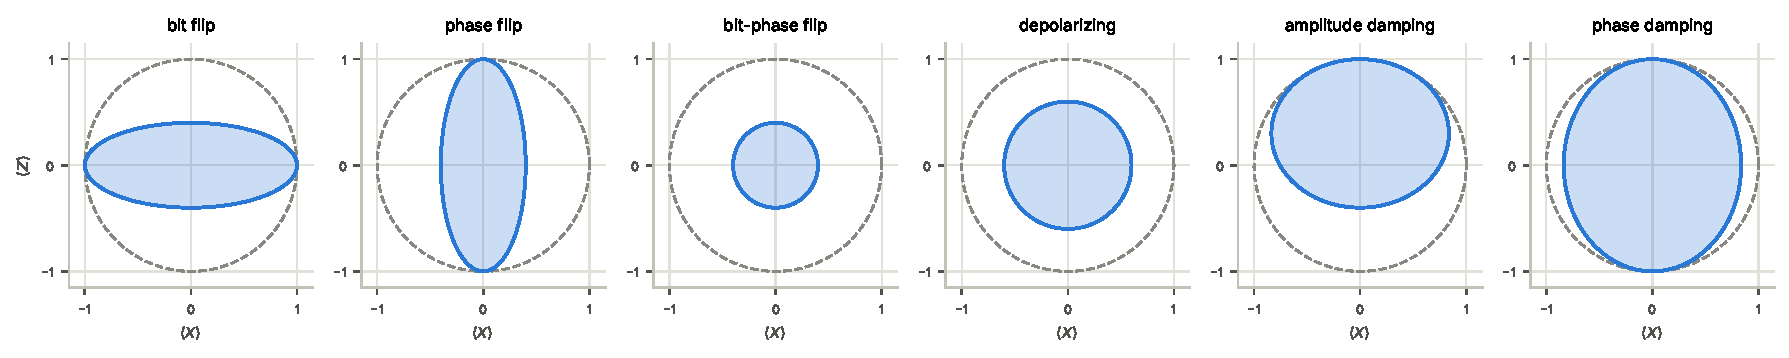
\includegraphics[width=\linewidth]{bloch_channels}\\
{\small $x$--$z$ section of the Bloch ball (dashed) and its image for $p = \gamma = \lambda = 0.3$: bit flip, phase flip, bit-phase flip, depolarizing,
amplitude damping, phase damping (illustrative experiment, checked with CUDA-Q).}
\end{center}
\begin{keyres}{phase errors are invisible in the $Z$ basis}
For a GHZ state with phase-flip noise the $Z$ population stays 1 while $\langle X^{\otimes N}\rangle$ drops (lecture: $0.0504$ at $p = 0.05$, 15 qubits, \texttt{stim}).
\end{keyres}

%=====================================================================================================
\section{Amplitude damping, phase damping, $T_1$ and $T_2$}
\begin{keyres}{damping channels}
Amplitude damping: $\rho_{11} \to (1-\gamma)\rho_{11}$, $\rho_{00} \to \rho_{00} + \gamma\rho_{11}$, $\rho_{01} \to \sqrt{1-\gamma}\rho_{01}$; non-unital.
Phase damping: $\rho_{01} \to \sqrt{1-\lambda}\rho_{01}$, populations fixed; equal to a phase flip with $1 - 2p = \sqrt{1-\lambda}$.
\end{keyres}
\begin{keyres}{relaxation times}
$\rho_{11}(t) = \rho_{11}(0)e^{-t/T_1}$; $|\rho_{01}(t)| = |\rho_{01}(0)|e^{-t/T_2}$; $\frac1{T_2} = \frac1{2T_1} + \frac1{T_\varphi}$, so $T_2 \le 2T_1$. Per step $\Delta t$:
$\gamma = 1 - e^{-\Delta t/T_1}$, $\sqrt{1-\lambda} = e^{-\Delta t/T_\varphi}$.
\end{keyres}
\begin{wexample}{an idling qubit}
$T_1 = 80$, $T_2 = 60\,\mu$s, $\ket+$, $t = 20\,\mu$s: $\rho_{11} = 0.389$, $|\rho_{01}| = 0.358$, $F(\ket+) = 0.858$, $T_\varphi = 96\,\mu$s.
Coherence-limited depth: $T_2 = 100\,\mu$s, 50 ns gates, coherence $\ge0.9$: 210 gates.
\end{wexample}
\begin{center}
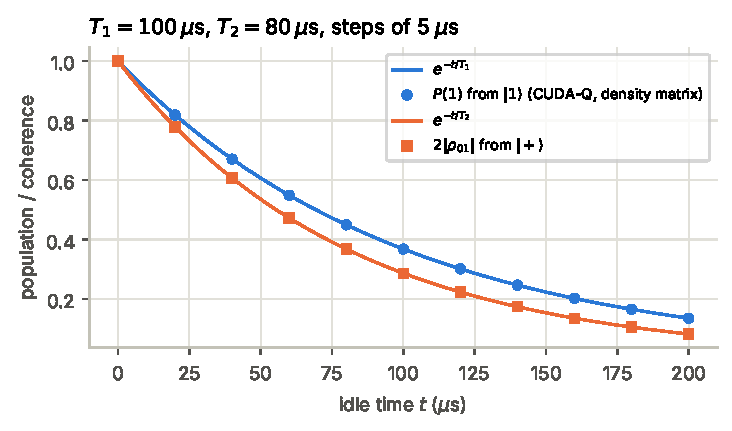
\includegraphics[width=0.75\linewidth]{t1t2}\\
{\small Repeated amplitude + phase damping steps reproduce $e^{-t/T_1}$ and $e^{-t/T_2}$ (CUDA-Q density matrix, illustrative).}
\end{center}
\begin{trap}
Scaling coherence by $1 - \gamma$ instead of $\sqrt{1-\gamma}$; adding $T$'s instead of rates; multiplying a $T_2$ decay by an extra $T_1$ factor.
\end{trap}

%=====================================================================================================
\section{Measurement errors}
$\mathbf q = A\mathbf p$ with $A_{ij} = P(\text{read }i\,|\,\text{state }j)$. $P(1|0) = 0.02$, $P(0|1) = 0.05$: $\ket+$ is read as 1 with probability $0.485$; a perfect 3-qubit
GHZ shows population $\frac12(0.98^3 + 0.95^3) = 0.899$. Mitigation: solve $A\mathbf p = \mathbf q$; e.g.\ $q_0 = 0.6$ gives $p_0 = 0.591$. Readout noise is
\emph{not} part of the notebook's noise model.

%=====================================================================================================
\section{Coherent and stochastic errors}
\begin{keyres}{accumulation}
Over-rotation $\varepsilon$ per gate: $P(\text{error}) = \sin^2\frac{n\varepsilon}{2}$ after $n$ gates (quadratic). Stochastic flip with $p = \sin^2\frac\varepsilon2$:
$\frac12[1 - (1-2p)^n] \approx np$ (linear). $\varepsilon = 0.05$, $n = 60$: $0.995$ vs.\ $0.036$. Pauli twirling turns coherent errors into Pauli channels.
\end{keyres}

%=====================================================================================================
\section{Simulating noise with CUDA-Q}
\begin{center}\small
\begin{tabularx}{\linewidth}{@{}llX@{}}\toprule method & target & properties\\ \midrule
density matrix & \texttt{density-matrix-cpu} & exact $\rho$, any channel, $16\cdot4^N$ bytes ($N = 13$: 1.07 GB)\\
trajectories & \texttt{nvidia} + noise model & statistical, $16\cdot2^N$ per trajectory, GPU (not run here)\\
stabilizer & \texttt{stim} & Clifford + Pauli noise only, hundreds of qubits\\ \bottomrule\end{tabularx}
\end{center}
\begin{trap}
(1) A constant \texttt{rx(0.0, q)} is removed by the compiler, so the noise attached to it never acts --- pass the angle as an argument.
(2) Keep a reference to the \texttt{NoiseModel} while CUDA-Q uses it (a temporary passed to \texttt{set\_noise} crashed the process).
(3) Noiseless targets ignore noise models. (4) \texttt{get\_state} has no \texttt{noise\_model} argument in CUDA-Q 0.16: use \texttt{set\_noise}.
\end{trap}

%=====================================================================================================
\section{The notebook and its results}
\begin{defn}{\texttt{build\_noise\_model(kind, p)}}
Single-qubit channel after \texttt{h}, \texttt{x}, \texttt{ry}, \texttt{rz}; two-qubit channel after every CNOT (\texttt{num\_controls=1}): \texttt{Depolarization2}, or
\texttt{Pauli2} with $p(1-p), p(1-p), p^2$ (independent flips), or the product Kraus set for amplitude damping. \texttt{auto}: GPU $\to$ trajectories;
CPU + GHZ + Pauli $\to$ \texttt{stim}; otherwise density matrix. Density-matrix counts are drawn from $\operatorname{diag}\rho$ with a seeded multinomial.
\end{defn}
\begin{center}
\begin{quantikz}[row sep=0.25cm, column sep=0.45cm]
\lstick{$\ket0$} & \gate{H} & \gate[style={fill=orange!20}]{\E} & \ctrl{1} & \gate[2,style={fill=orange!20}]{\E_2} & \qw & \qw & \meter{}\\
\lstick{$\ket0$} & \qw & \qw & \targ{} & & \ctrl{1} & \gate[2,style={fill=orange!20}]{\E_2} & \meter{}\\
\lstick{$\ket0$} & \qw & \qw & \qw & \qw & \targ{} & & \meter{}
\end{quantikz}\\
{\small The notebook's GHZ circuit with its noise locations (3 qubits shown; the default has 15).}
\end{center}
\begin{center}
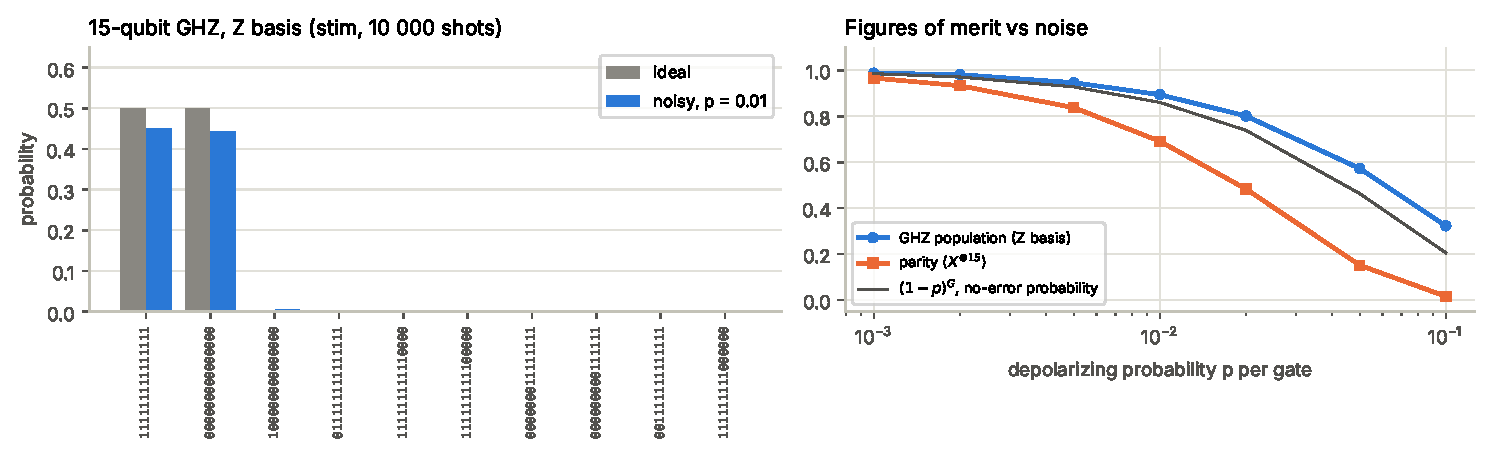
\includegraphics[width=\linewidth]{ghz_sweep}\\
{\small Re-executed default run: ideal vs.\ noisy distribution and figures of merit vs.\ $p$ (identical to the recorded outputs).}
\end{center}
\begin{wexample}{the recorded run (re-executed identically)}
Depolarizing, \texttt{stim}: $p = 0.01$: population $0.8936$, parity $0.6910$, $(1-p)^{15} = 0.8601$, 96 outcomes; $p = 0.1$: $0.3232$, $0.0160$, 1165 outcomes.
Leaked probability $1 - 0.8936 = 0.1064$. Bit-flip no-error probability $(1-p)^{29} = 0.7472$ at $p = 0.01$.
\end{wexample}
\begin{keyres}{figures of merit}
Hellinger $F_H = (\sum\sqrt{p_xq_x})^2$ (equal to the population for a balanced two-peak ideal), TVD $\frac12\sum|p_x - q_x|$, parity $P(\text{even}) - P(\text{odd})$,
state fidelity and purity (density matrix only). $(1-p)^G$ is a lower bound for Pauli noise, not the exact fidelity: 6-qubit GHZ at $p = 0.01$ has $F = 0.9492 > 0.99^6 = 0.9415$.
\end{keyres}

%=====================================================================================================
\section{Fidelity measures and benchmarking}
$F_{\text{avg}} = \frac{dF_{\text{pro}} + 1}{d + 1}$; depolarizing qubit: $F_{\text{pro}} = 1 - p$, $F_{\text{avg}} = 1 - \frac{2p}{3}$. Randomized benchmarking:
$A\alpha^m + B$, $r = \frac{(d-1)(1-\alpha)}{d}$ ($\alpha = 0.99 \Rightarrow r = 0.005$). Both are theory only in this repository.

%=====================================================================================================
\section{Error mitigation}
\begin{keyres}{zero-noise extrapolation}
Linear $2E(1) - E(2)$; Richardson $3E(1) - 3E(2) + E(3)$; exponential $E(1)^2/E(2)$. Folding $G \to GG^\dagger G$: fold 4 of 10 gates $\Rightarrow\lambda = 1.8$.
Lecture example (4-qubit GHZ parity, $p = 0.01\lambda$): $0.9055, 0.8189, 0.7396 \Rightarrow$ linear $0.9921$, Richardson $0.9994$, exponential $1.0021$ (overshoot).
\end{keyres}
\begin{trap}
ZNE and readout mitigation estimate expectation values --- they do not repair the state, they cost extra shots, and they are model dependent.
\end{trap}

%=====================================================================================================
\section{Dynamical decoupling and error correction}
\begin{keyres}{echo}
Static detuning: free decay $e^{-\sigma^2t^2/2}$ ($\sigma = 1$, $t = 2$: $0.135$); Hahn echo restores 1 because $XR_Z(a)X = R_Z(-a)$. Independent phase flips per step
($p = 0.02$, 20 steps): $0.96^{20} = 0.442$ with and without echo.
\end{keyres}
\begin{center}
\begin{quantikz}[row sep=0.2cm, column sep=0.35cm]
\lstick{$\ket\psi$} & \ctrl{1} & \ctrl{2} & \gate[3,style={fill=orange!20}]{X\text{ w.p. }p} & \ctrl{1} & \ctrl{2} & \targ{} & \qw\\
\lstick{$\ket0$} & \targ{} & \qw & & \targ{} & \qw & \ctrl{-1} & \qw\\
\lstick{$\ket0$} & \qw & \targ{} & & \qw & \targ{} & \ctrl{-1} & \qw
\end{quantikz}\\
{\small Encode, bit flips, decode and majority vote (Toffoli).}
\end{center}
\begin{keyres}{bit-flip code}
$P_L = 3p^2 - 2p^3$ (0.028 at $p = 0.1$); useful for $p < \frac12$. Surface code $p_L \propto (p/p_{\text{th}})^{(d+1)/2}$: $d = 3 \to 5$ at $p/p_{\text{th}} = 0.1$ gains $\times10$.
\end{keyres}

%=====================================================================================================
\section{Problem-solving strategies and question map}
\begin{method}{five habits}
\begin{enumerate}[itemsep=1pt]
\item \textbf{Convention first}: which depolarizing $p$? Which qubit first? Probability or amplitude?
\item \textbf{Go to the Bloch vector}: every single-qubit channel is an affine map of $\vec r$.
\item \textbf{Populations vs.\ coherences}: $T_1$/amplitude damping move populations; phase noise only coherences.
\item \textbf{Count locations}: one per gate for joint channels, two per CNOT for independent flips.
\item \textbf{Simulation $\neq$ mitigation $\neq$ correction $\neq$ hardware}.
\end{enumerate}
\end{method}
\begin{center}\small
\begin{tabularx}{\linewidth}{@{}lX@{}}
\toprule Section & Assessment questions\\ \midrule
1 Error statistics & 7, 8, 13, 30, 31\\
2 Density matrices & 1, 2, 3, 4, 12, 14, 15, 17, 18, 19, 20\\
3 Decoherence, fidelity & 6, 10, 11, 32\\
4 Channels, CPTP & 5, 16, 35, 43, 44, 45\\
5 Pauli channels & 21, 22, 23, 33, 34, 36, 38, 41\\
6 Damping, $T_1$, $T_2$ & 24, 25, 26, 27, 28, 29, 37, 39, 40\\
7 Measurement errors & 30, 31, 66, 67\\
8 Coherent vs.\ stochastic & 9, 32, 72, 73\\
9 CUDA-Q simulation & 41, 42, 48, 49, 53, 54, 55, 58, 74\\
10 Notebook and results & 46, 47, 50, 51, 52, 56, 57, 59, 60, 78\\
11 Fidelity, benchmarking & 61, 62\\
12 Error mitigation & 63, 64, 65, 66, 67, 77, 79, 80\\
13 DD and QEC & 68, 69, 70, 71, 75, 76\\ \bottomrule
\end{tabularx}
\end{center}

%=====================================================================================================
\section{Practice problems}
Try each before looking at the answers on the next page.
\begin{enumerate}[label=\textbf{P\arabic*.}, leftmargin=2.6em, itemsep=3pt]
\item Bloch vector and purity of $\begin{psmallmatrix}0.75 & 0.25\\ 0.25 & 0.25\end{psmallmatrix}$.
\item Depolarizing (CUDA-Q) $p = 0.15$ on $\ket+$: $\langle X\rangle$ and $P(-)$.
\item Amplitude damping $\gamma = 0.19$ on $\ket+$: the output density matrix.
\item The phase-flip probability equivalent to phase damping with $\lambda = 0.19$.
\item $T_1 = 40\,\mu$s; a qubit starts in $\ket1$. $P(1)$ after $20\,\mu$s?
\item $T_1 = 60\,\mu$s, $T_2 = 40\,\mu$s: $T_\varphi$?
\item $P(1|0) = 0.03$, $P(0|1) = 0.08$: probability that $\ket{11}$ is read correctly.
\item Bit flip $p = 0.25$ on $\ket0$: output and purity.
\item Notebook GHZ with 10 qubits at $p = 0.02$: no-error probability for depolarizing and for bit-flip noise.
\item Density-matrix memory for 11 qubits.
\item ZNE: $E(1) = 0.90$, $E(2) = 0.82$. Linear estimate?
\item Bit-flip code at $p = 0.2$: logical error.
\item Readout calibration $P(0|0) = 0.97$, $P(0|1) = 0.06$; measured $q_0 = 0.5$. Mitigated $p_0$?
\item Average gate fidelity of a depolarizing qubit channel with $p = 0.006$.
\end{enumerate}

\newpage
\subsection*{Answers to the practice problems}
\begin{enumerate}[label=\textbf{P\arabic*.}, leftmargin=2.6em, itemsep=3pt]
\item $\vec r = (0.5, 0, 0.5)$; purity $\frac{1 + 0.5}{2} = 0.75$.
\item $\langle X\rangle = 1 - \frac{4(0.15)}{3} = 0.8$; $P(-) = 0.1$.
\item $\begin{psmallmatrix}0.595 & 0.45\\ 0.45 & 0.405\end{psmallmatrix}$ ($\rho_{00} = 0.5 + 0.19\cdot0.5$, $\rho_{01} = 0.9\cdot0.5$).
\item $1 - 2p = \sqrt{0.81} = 0.9 \Rightarrow p = 0.05$.
\item $e^{-0.5} = 0.607$.
\item $\frac1{T_\varphi} = \frac1{40} - \frac1{120} = \frac1{60}$: $T_\varphi = 60\,\mu$s.
\item $0.92^2 = 0.8464$.
\item $\operatorname{diag}(0.75, 0.25)$; purity $0.5625 + 0.0625 = 0.625$.
\item Depolarizing $0.98^{10} = 0.817$; bit flip $0.98^{19} = 0.681$.
\item $16\cdot4^{11} = 67.1$ MB.
\item $2(0.90) - 0.82 = 0.98$.
\item $3(0.04) - 2(0.008) = 0.104$.
\item $p_0 = \frac{0.5 - 0.06}{0.97 - 0.06} = 0.484$.
\item $1 - \frac{2(0.006)}{3} = 0.996$.
\end{enumerate}

\subsection*{Summary of the chapter in ten lines}
\begin{enumerate}[itemsep=1pt]
\item Errors multiply: $(1-p)^G$; shot noise $\sqrt{P(1-P)/S}$.
\item $\rho = \frac12(I + \vec r\cdot\vec\sigma)$; purity $\frac{1 + |\vec r|^2}{2}$; mixed $\Leftrightarrow$ inside the ball.
\item Decoherence = entanglement with the environment = random phases on average.
\item Channels: $\sum K\rho K^\dagger$, $\sum K^\dagger K = I$; Kraus sets not unique.
\item Bit/phase/bit-phase flip keep one axis; depolarizing shrinks by $1 - \frac{4p}{3}$.
\item Amplitude damping shifts towards $\ket0$ ($T_1$); phase damping $\leftrightarrow$ $T_\varphi$; $\frac1{T_2} = \frac1{2T_1} + \frac1{T_\varphi}$.
\item Readout errors: $\mathbf q = A\mathbf p$; coherent errors grow quadratically, stochastic linearly.
\item CUDA-Q: \texttt{stim} (Clifford + Pauli), density matrix ($4^N$), trajectories ($2^N$, GPU); keep the model alive; avoid constant identities.
\item The notebook's sweep is reproduced exactly; $(1-p)^G$ is a bound, parity reveals phase errors.
\item Mitigation estimates, DD refocuses slow noise, QEC protects --- and none of this here ran on hardware.
\end{enumerate}
\end{document}
